\subsubsection{Waste Form Degradation Rate and Contaminant Inventory Sensitivity}

In the parametric sensitivity analysis discussed in Section 
\ref{sec:wfdeginv}, the results showed two regimes. In the first regime, 
the mean of the peak annual dose rates is directly proportional to both the mass 
factor and the fractional waste form degradation rate. For some radionuclides, 
attenuation occurs for high values of both parameters as the release of 
radionuclides is limited by dispersion parameters. This phenomenon can be seen 
in the figures below in which transition between regimes for higher degradation 
rates happens at lower mass factors than transition between regimes for lower 
degradation rates. 

The peaks for highly soluble, non sorbing elements such as $I$ and $Cl$
are directly proportional to mass factor for most 
values of waste form degradation rates. This effect can be seen in Figures 
\ref{fig:WFDegI129}, \ref{fig:WFDegI129MF}, \ref{fig:WFDegCl36}, and 
\ref{fig:WFDegCl36MF}. 


Highly soluble and non-sorbing $^{129}I$ demonstrates a direct proportionality between dose rate and 
fractional degradation rate until a turnover where other natural system 
parameters dampen transport. Highly soluble and non-sorbing $^{129}I$ domonstrates a direct 
proportionality to the inventory multiplier.

\begin{figure}[ht!]
\begin{minipage}[b]{0.45\linewidth}
\centering
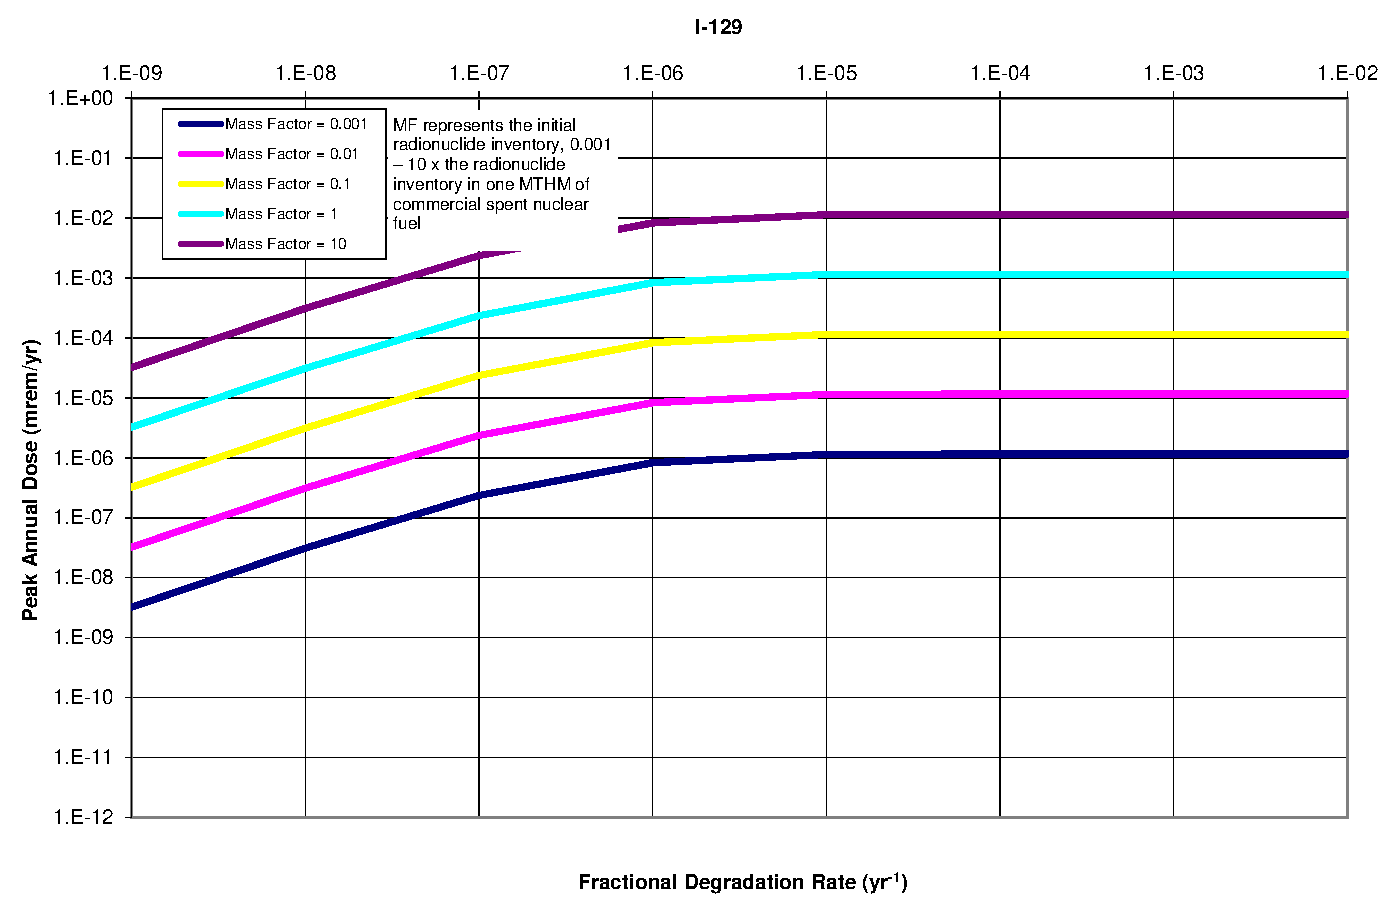
\includegraphics[width=\linewidth]{./chapters/nuclide_sensitivity/clay/WFDegAndInv/I-129.eps}
\caption{$^{129}I$ waste form degradation rate sensitivity.}
\label{fig:WFDegI129}

\end{minipage}
\hspace{0.05\linewidth}
\begin{minipage}[b]{0.45\linewidth}

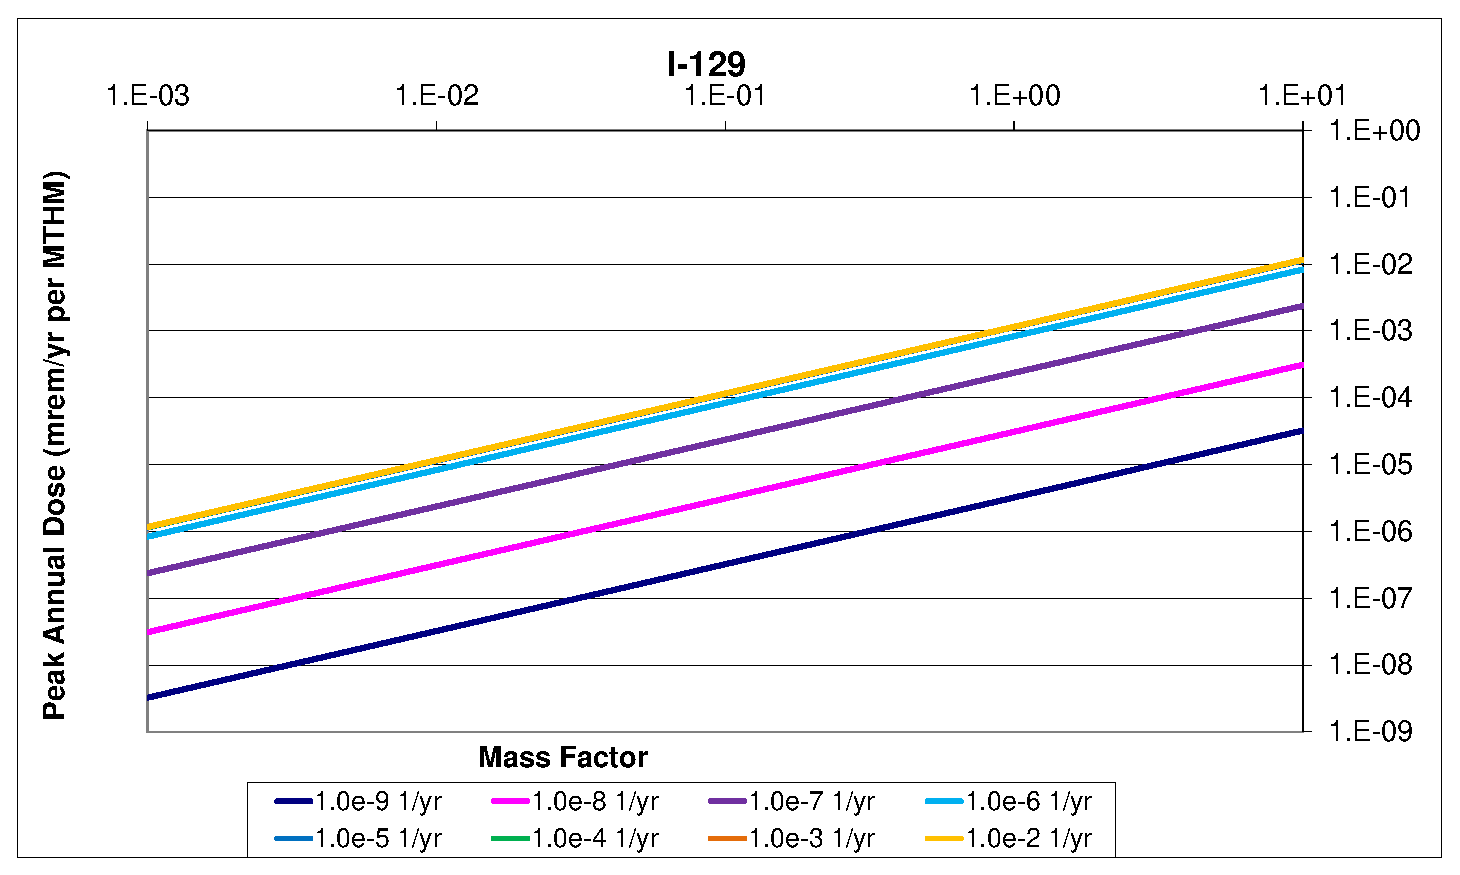
\includegraphics[width=\linewidth]{./chapters/nuclide_sensitivity/clay/WFDegAndInv/I-129-MF.eps}
\caption{$^{129}I$ inventory multiplier sensitivity.}
\label{fig:WFDegI129MF}

\end{minipage}
\end{figure}
\begin{figure}[ht]
\begin{minipage}[b]{0.45\linewidth}

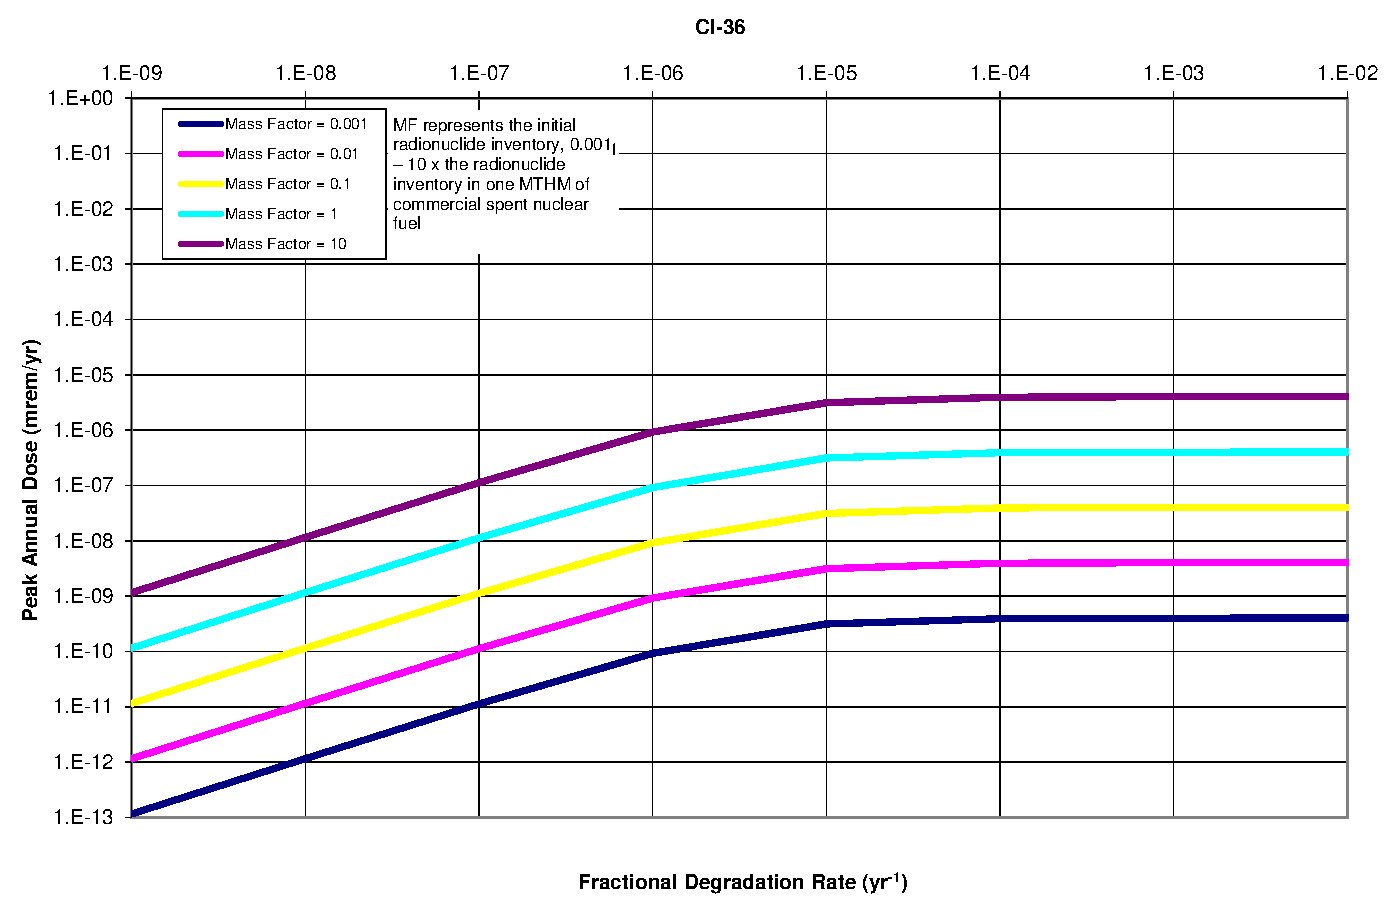
\includegraphics[width=\linewidth]{./chapters/nuclide_sensitivity/clay/WFDegAndInv/Cl-36.eps}
\caption{$^{36}Cl$ waste form degradation rate sensitivity.}
\label{fig:WFDegCl36}

\end{minipage}
\hspace{0.05\linewidth}
\begin{minipage}[b]{0.45\linewidth}

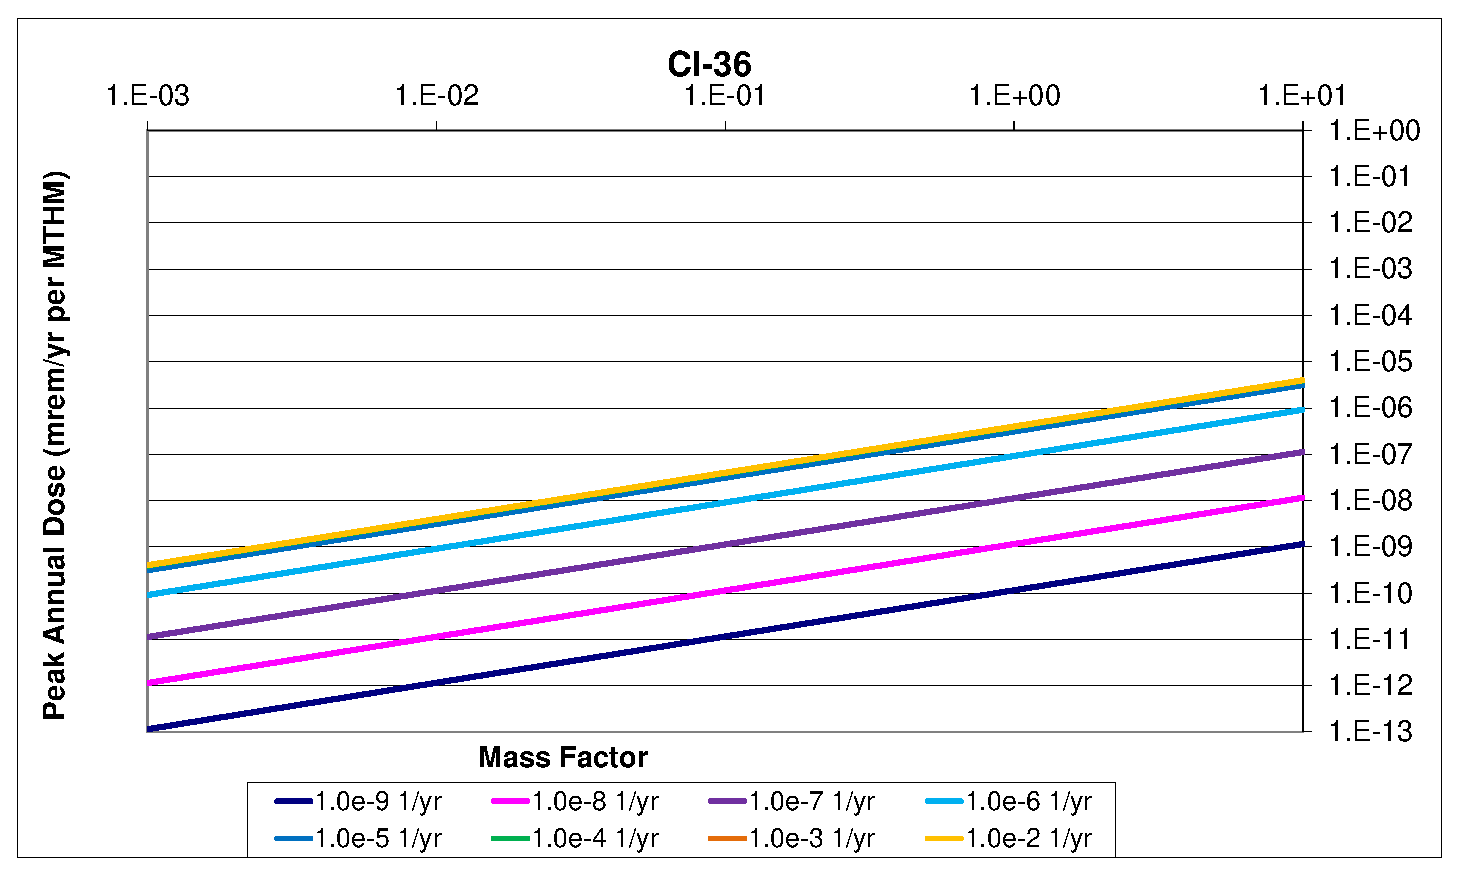
\includegraphics[width=\linewidth]{./chapters/nuclide_sensitivity/clay/WFDegAndInv/Cl-36-MF.eps}
\caption{$^{36}Cl$ inventory multiplier sensitivity.}
\label{fig:WFDegCl36MF}
\end{minipage}
\end{figure}

The peaks for solubility limited, sorbing elements such as $Tc$ and $Np$, on the 
other hand, have a more dramatic turnover.  For very high degradation rates, the 
dependence on mass factor starts to round off due to attenuation by solubility 
limits, as can be seen in Figures \ref{fig:WFDegNp237}, \ref{fig:WFDegNp237MF}, 
\ref{fig:WFDegTc99}, and \ref{fig:WFDegTc99MF}.

Solubility limited and sorbing $^{99}Tc$ demonstrates a direct proportionality 
to fractional degradation rate until attuation by its solubility limit and other 
natural system parameters.  

\begin{figure}[ht!]
\begin{minipage}[b]{0.45\linewidth}

\centering
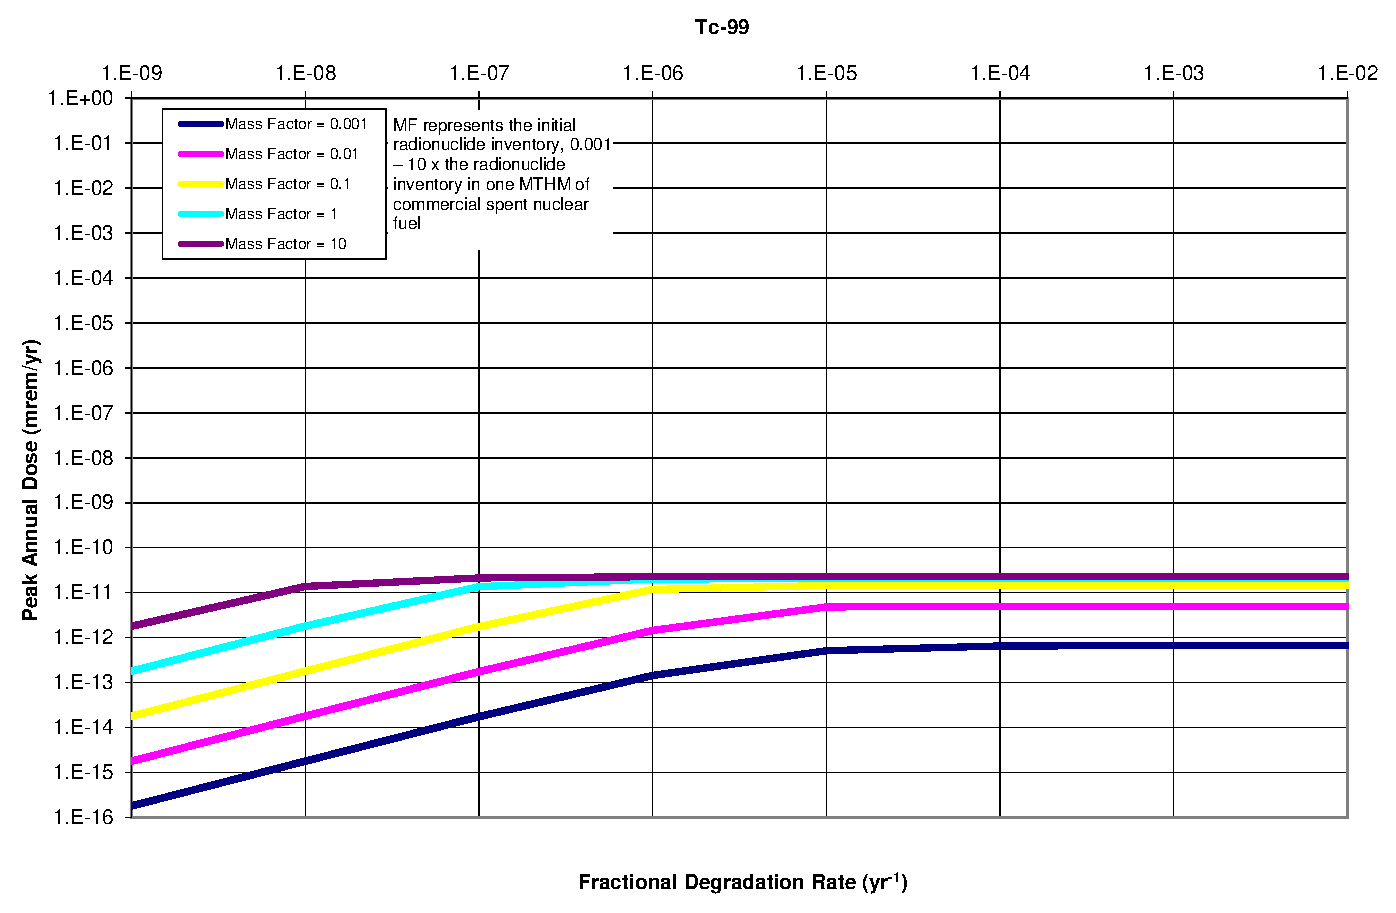
\includegraphics[width=\linewidth]{./chapters/nuclide_sensitivity/clay/WFDegAndInv/Tc-99.eps}
\caption{$^{99}Tc$ waste form degradation rate sensitivity.}
\label{fig:WFDegTc99}

\end{minipage}
\hspace{0.05\linewidth}
\begin{minipage}[b]{0.45\linewidth}

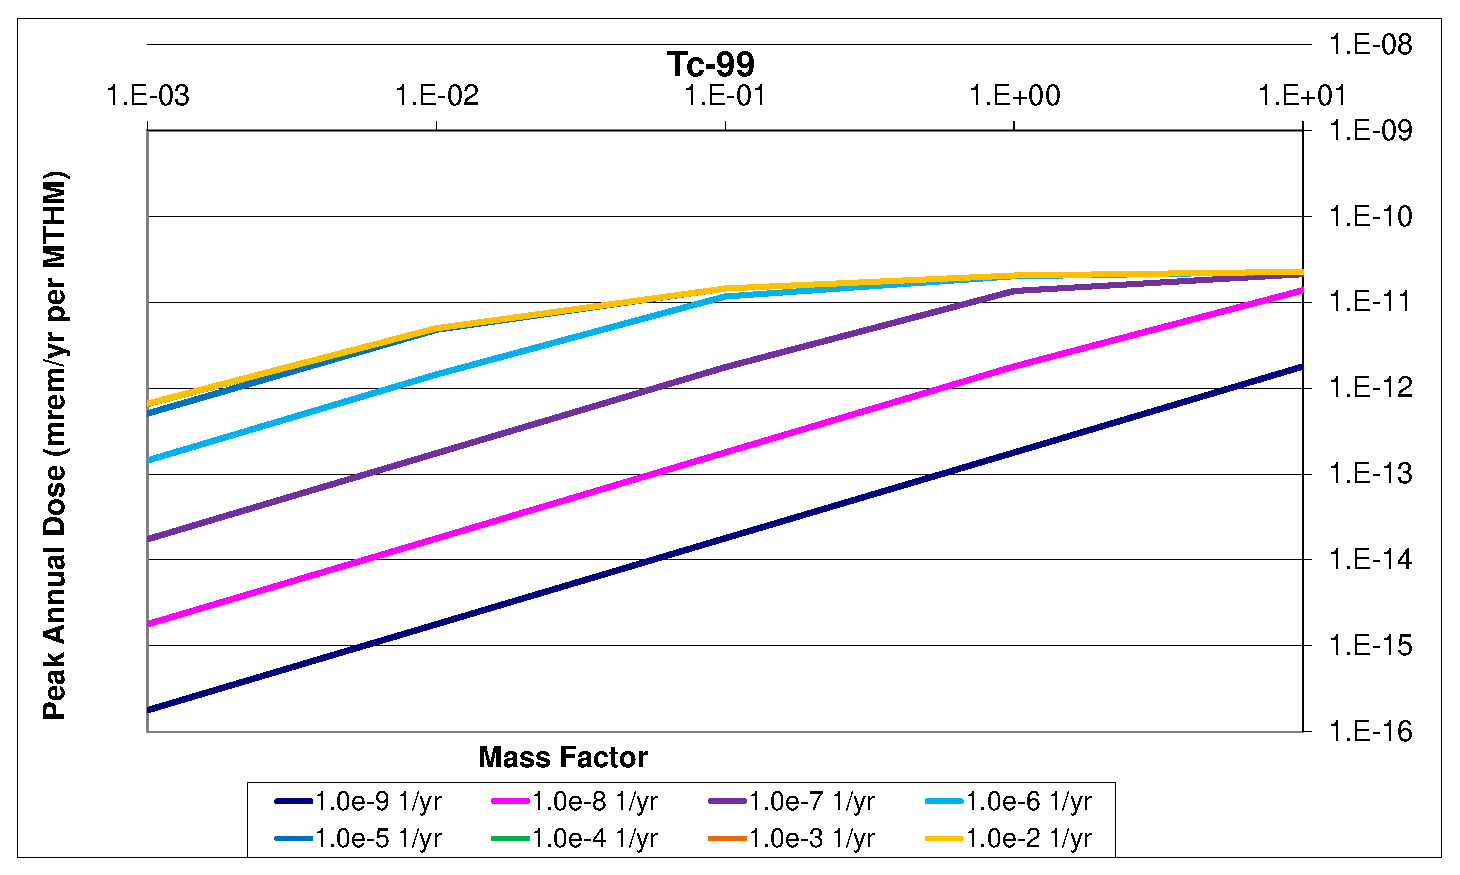
\includegraphics[width=\linewidth]{./chapters/nuclide_sensitivity/clay/WFDegAndInv/Tc-99-MF.eps}
\caption{$^{99}Tc$ inventory multiplier sensitivity.}
\label{fig:WFDegTc99MF}

\end{minipage}
\end{figure}
\begin{figure}[ht]
\begin{minipage}[b]{0.45\linewidth}

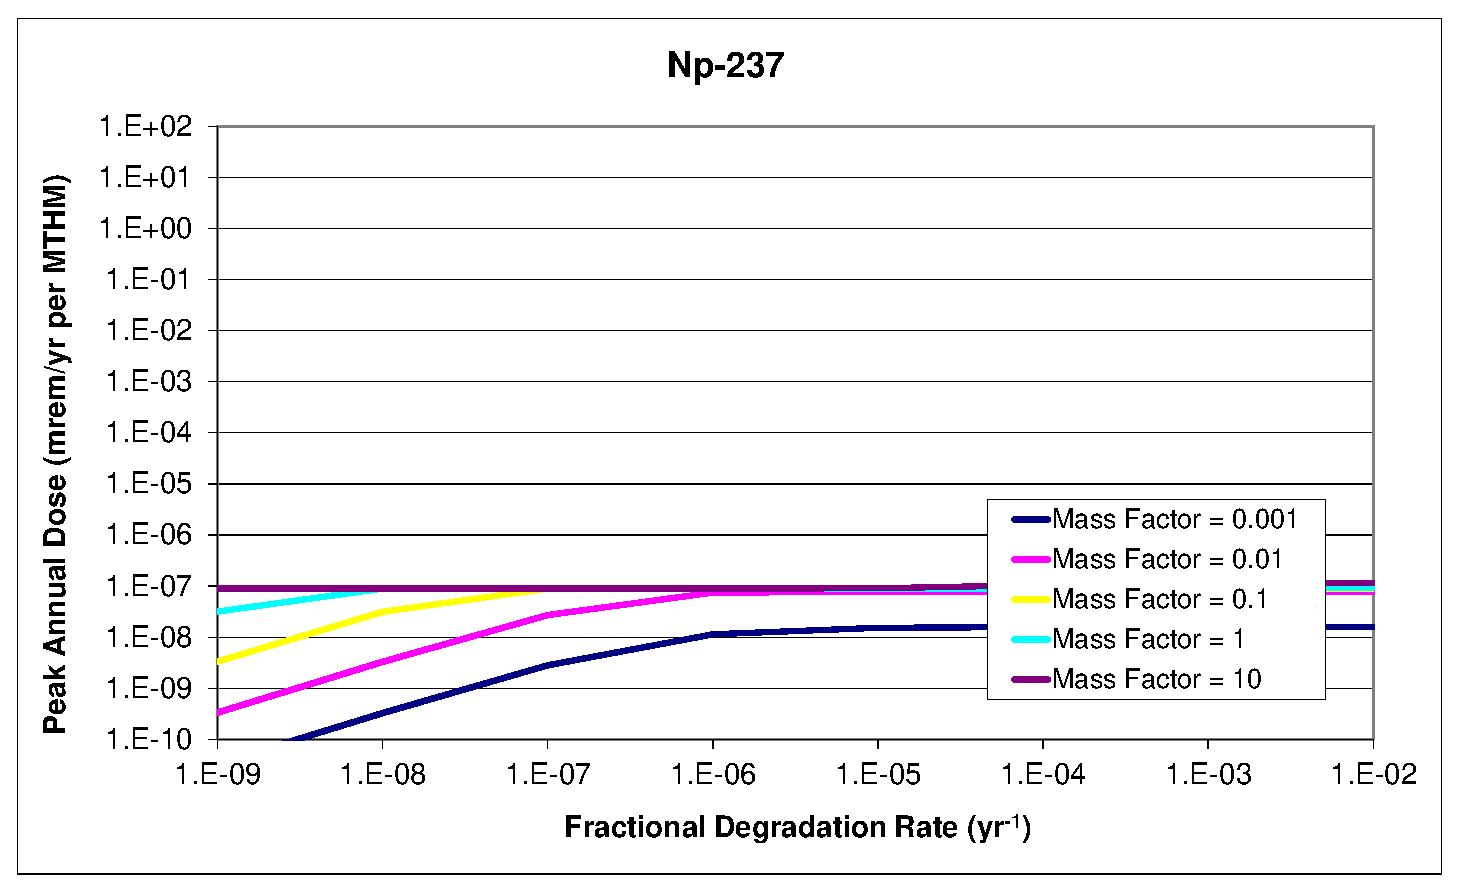
\includegraphics[width=\linewidth]{./chapters/nuclide_sensitivity/clay/WFDegAndInv/Np-237.eps}
\caption{$^{237}Np$ waste form degradation rate sensitivity.}
\label{fig:WFDegNp237}

\end{minipage}
\hspace{0.05\linewidth}
\begin{minipage}[b]{0.45\linewidth}

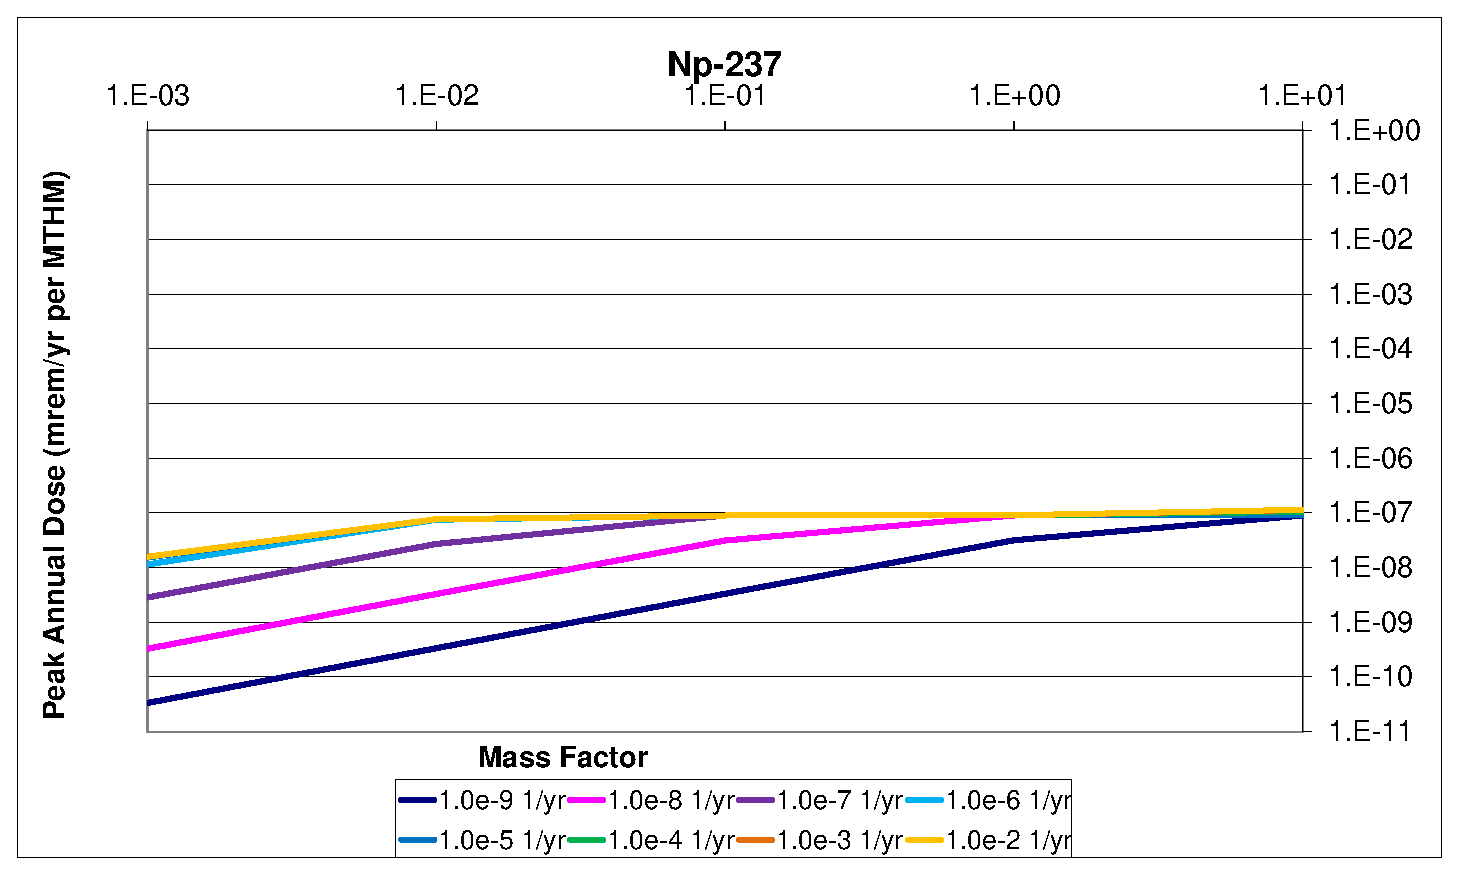
\includegraphics[width=\linewidth]{./chapters/nuclide_sensitivity/clay/WFDegAndInv/Np-237-MF.eps}
\caption{$^{237}Np$ inventory multiplier sensitivity.}
\label{fig:WFDegNp237MF}

\end{minipage}
\end{figure}
\clearpage 
